\chapter{Related Work}
\label{cha:Related Work}

This thesis will reinforcement learning in the training of an autonomous driving agent that utilizes a convolutional neural network to process visual input. The approach used in this thesis differs greatly from previous work at the ScaDS.AI \autocite{maximilian} both in the agent design and training setup. Therefore research relating to reinforcement learning algorithms, convolutional neural networks and self-driving will be reviewed. 
% also research regarding rebustness to light changes?

% TODO auch die Ergebnisse der Paper und die daraus gezogenenn Schlüsselideen erwähnen


\section{Reinforcement Learning}

Reinforcement Learning algorithms have been around for a long time, but only recently have they been able to achieve superhuman performance in games and control tasks \autocite{atari}. Most reinforcement learning algorithms formalize the problem as consisting of an environment and an agent. The environment consists of a state space and an action space and a reward function that takes state-action pairs as input. Reward functions assign positive rewards to actions that are deemed to be desirable by the algorithm designers, for example scoring a goal in a football match. Reward function can also assign negative rewards to undesirable actions, for example collisions in a driving simulation. The agent processes the environment, takes actions and observes the assigned reward. The observed rewards are then used to update the policy \ref{rlcycle}. RL algorithms train the agent to select an action in a given state and maximize the cumulative reward along the state transitions. The process of selecting an action is called the policy $\pi$ \autocite{rlbook2020}. 

\begin{figure}
    \centering
    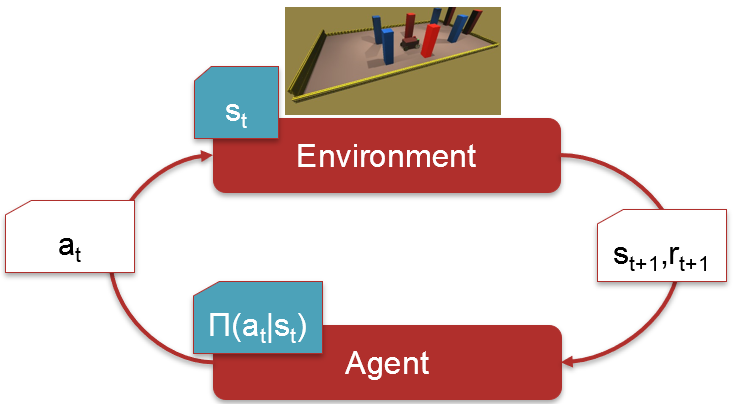
\includegraphics[width=0.4\textwidth]{Bilder/rl_cycle.png}
    \caption{RL Training Cycle: The agent selects action $a_t$ based on policy $\pi(a_t|s_t)$ at state $s_t$ and recieves the next state $s_{t+1}$ and rewards $r_{t+1}$ from the environment. Observed rewards are used to update the policy.}
    \label{rlcycle}
\end{figure}

Reinforcement learning algorithms are classified into two major groups. RL algorithms that use a model of the environment are called model-based algorithms, algorithms without such models are called model-free algorithms. Algorithms from both groups have been successfully used in a wide range of applications, model-based algorithms are often much more complex but have been shown to be successful at many task that require planning \autocite{alphagoimprovementmuzero}. Model-free approaches are often simpler and more flexible, they have shown great success in various control tasks \autocite{atari}.

\begin{figure}
    \centering
    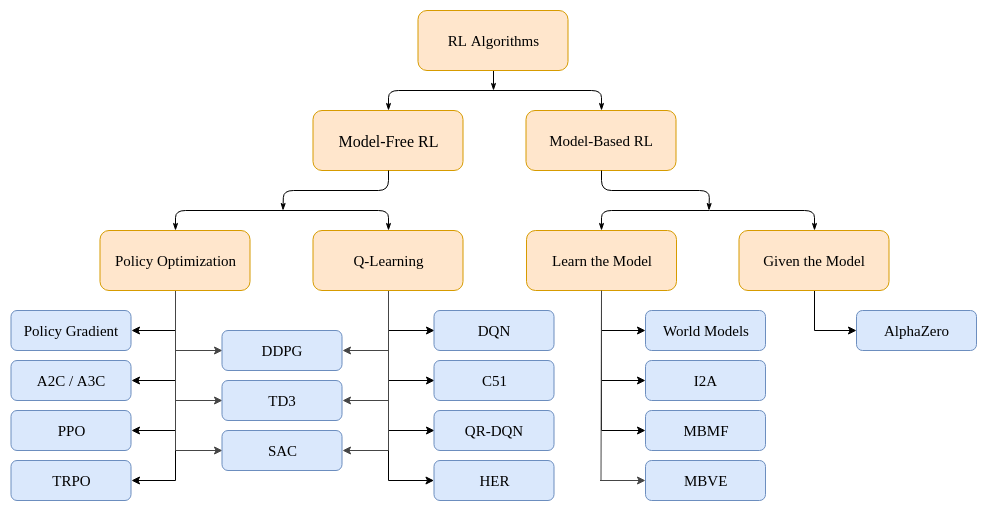
\includegraphics[width=0.8\textwidth]{Bilder/openai_spinningup_taxonomy.png}
    \caption{Taxonomy of RL algorithms from OpenAI's Spinning Up course \autocite{spinningup}}
\end{figure}
% TODO is this citation correct?

Early implementations of RL algorithms used functions with a discrete input space for their policy such as for example tables that store state-action pairs and associated values. These algorithms belong to the family of value-based algorithms and include Q-learning and deep-Q learning. In Q-learning, the trained policy function takes a state as input, searches the state in the table and selects the associated action with the highest value. For many problems the use of these tables in not feasible due to the amount of state-action pairs, many extensions to the algorithms have been developed such as for example deep-Q network (DQN). DQN uses a deep (convolutional) neural network to approximate the Q-values \autocite{atari}.
Although they have been used to great success for control tasks they will not be used in this thesis, as they require discrete action spaces and the environment in this thesis consists of a continuous action space.


The other family are policy-based algorithms, instead of learning the values associated to state-action pairs these algorithms learn the policy directly. This allows for the use of continuous action spaces. The Proximal Policy Optimization algorithm was developed to improve the stability of policy-based algorithms \autocite{ppo}. The PPO algorithm restricts the size of policy changes caused by parameter updates, which ensures the policy cannot change drastically and improves stability. PPO is currently one of the most popular algorithms for reinforcement learning, and has already been successfully used in the domain of autonomous driving \autocite{maximilian}. The PPO algorithm can be used with convolutional neural networks as well and will therefore be used in this thesis.


% Another major improvement in the domain of reinforcement learning was the combination of neural networks with traditional planning and search algorithms, the most famous example for this is AlphaGo \autocite{alphago}. These algorithms often are model-based algorithms and use search algorithms (e.g. Monte Carlo Tree Search)  to evaluate the possible actions at a given state. The neural networks are used for the evaluation of states and actions in the search algorithms. AlphaGo was developed for a 2 player deterministic game with a discrete state and action space. Since then this combination of neural networks and search algorithms has also been used to achieve impressive results for all kinds of problems \autocite{alphafold}, for example single player continuous state and action spaces \autocite{alphagoimprovementmuzero}. Although these algorithms could be applied to the problem at hand, they will not be utilized due to the increased complexity of the algorithms and the required computational resources.
% TODO sollte der Teil wieder rein?


\subsection*{Convolutional Neural Network for Reinforcement Learning}

Convolutional neural networks are a neural network architecture specifically developed for processing image data, they consist of a number of filters and a fully connected neural network. The filters are applied to the image in a sliding window fashion, the filters detect patterns in the image such as for example edges and corners. Multiple successive applications of such filters enables the network to learn hierarchical information and recognize more complex structures. The fully connected neural network analyses the results of the filters and makes the final prediction \autocite{rlbook2020}.

CNNs are often used in Reinforcement Learning since RL problems often require an agent to process visual input. Furthermore CNNs can be trained end-to-end in Reinforcement Learning compared to other feature extraction methods, which means the CNN can learn what features are important for the task at hand.
Therefore a convolutional neural network will be used to process the camera images instead of a hand-crafted feature extraction method. 

CNNs typically do not take the raw camera/simulation images but rather preprocessed images, e.g. greyscaled images \autocite{atari}. Preprocessing steps can help in reducing the complexity of the input space. Convolutional neural networks require a lot of data to learn, data augmentation can help increase the size of the training set and to make the agent more robust. Data augmentation generates new samples from already collected ones by applying transformations to the samples. 


% rlbook2020 chapter 9.7 explains the use of CNNs in RL


\section{Self-Driving}

As mentioned before, there has been a lot of progress in the domain of self-driving in recent years. Sophisticated self-driving algorithms often consist of many components to achieve satisfying performance, Tesla's self-driving for example uses separate object detection, occupancy and planning components that are built on top of convolutional neural networks \autocite{howteslaautopilot}. % (CNN is ResNet)
Self-driving in a real world environment is a very complex task, especially when including other traffic participants. It requires agents that consist of multiple complex components \autocite{drl_for_ad} and is beyond the scope of the thesis. Instead I aim to contribute to the domain by expanding on previous research and focus on the training of a convolutional neural network. Approaches from the domain of self-driving will be used to improve the training of the agent, for example reward shaping \autocite{drl_for_ad}.

This thesis builds directly upon the work of \autocite{jonas_koenig}, \autocite{merlin_flach} and \autocite{maximilian}. \autocite{jonas_koenig} built a self-driving agent that was trained to avoid collisions in a simulated arena using an evolutionary approach to neural network training. The agent used a preprocessing pipeline to extract information from visual input. The extracted features were given to a neural network policy. \autocite{merlin_flach} investigated the feasibility of transferring the agent to the real world. The research showcased many difficulties, most notably the object recognition part of the preprocessing pipeline. \autocite{maximilian} investigated a different task than the two previous papers, the agent was trained to pass a parcour by driving through a sequence of goals. This task is identical to the one investigated here. \autocite{maximilian} successfully used PPO to train the agent which also used a preprocessing pipeline similar to \autocite{jonas_koenig}.
The instability of the hand-crafted preprocessing pipeline and promissing results by CNNs from other RL researchers in the domain of self-driving \autocite{neptune} motivate the choice of CNNs as the feature extraction method in this thesis. 

%Another interesting approach to building self-driving agents is using imitation learning \autocite{imitation_learning}, imitation learning agents learn to mimic the behaviour exhibited in the training set. The training set is usually generated by humans driving the car, this approach is rumored to be used by Tesla to train their self-driving agents \autocite{teslaEndToEnd}.


% \autocite{autonomous_vehicles_review} %TODO read this paper and cite it

% https://safe-intelligence.fraunhofer.de/en/autonomous-driving

% Papers that use Carla



% Mention experiments from PopCulture/YouTube


\section{Simulation for Reinforcement Learning and Self-Driving}

% TODO Carla und andere Simulations machen keinen Sinn, da wir ein festse Problem haben

Simulations play a huge role in reinforcement learning and thus the development of self-driving agents. Simulations provide a huge number of benefits over real world experiments. They are much cheaper and faster to run than real world experiments, furthermore they can be run in parallel. In addition the programmers have direct and perfect control over the environment, as such programmers can for example change the simulation speed. This allows for fast experimentation and training of reinforcement learning agents. Simulations also allow for the creation of scenarios that are not possible in the real world. This is especially useful for reinforcement learning agents that are trained to avoid collisions. Simulations also allow for the creation of ground truths such as perfect sensor data and object bounding boxes \autocite{carla}.

Simulated environments often serve as baselines for reinforcement learning algorithms, most famous are the atari games \autocite{atari}. The Python Gynasium API was developed for easy reuse and comparison of reinforcement learning algorithms for different problems \autocite{gymnasium}, the Gymnasium API defines an interface that can be used to model tasks as reinforcement learning problems. A wide range of reinforcement learning frameworks support the Gymnasium API, for example Google's dopamine \autocite{dopamine} and OpenAI's baselines \autocite{sb3}. Advanced simulations like the Unity engine \autocite{unity}, the physics simulator MuJoCo \autocite{mujoco} and the driving simulator Carla \autocite{carla} can be integrated with the Gymnasium API.

%The complexity and interest in self-driving has also led to the development of dedicated simulators, such as the Carla \autocite{carla} and the AirSim \autocite{airsim} simulator. The Carla simulator provides researchers with useful features such as weather control and ground truths for object detection and segmentation.

There are also dedicated frameworks for reinforcement learning that directly integrate with simulation engines. \autocite{maximilian} used the ML-Agents framework \autocite{mlagents} to train the self-driving agent in Unity directly.

In this thesis Unity will be used for the simulation, the simulation will be integrated with the Python Gymnasium API and PPO algorithm. This approach is chosen instead of the ML-Agents framework since it allows for more flexibility and control over the simulation and training process.


% figure of unity ?


% TODO check Ray: https://docs.ray.io/en/latest/rllib/index.html
% TODO check dopamine https://github.com/google/dopamine


%\section{Reinforcement Learning for Self-Driving}

%\autocite{drl_for_ad} review the use of reinforcement learning for autonomous driving, they also describe many improvements for reinforcement learning algorithms that can improve the training stability and performance, such as for example reward shaping.
%In addition to published research papers there have been a lot of experiments, tutorials and demonstrations of self-driving agents on YouTube and GitHub. The University of Tübingen published their full lecture series on Self-Driving Cars \autocite{tuebingen}, the series also includes a section on reinforcement learning.

% papers that cite carla: https://scholar.google.de/scholar?cites=660591080772510291&as_sdt=2005&sciodt=0,5&hl=de


% Tübingen: % https://www.youtube.com/watch?v=GYnlqiSqZiU&list=PL05umP7R6ij321zzKXK6XCQXAaaYjQbzr&index=13



% Key Papers in RL: https://spinningup.openai.com


